\documentclass{article}

%other packages
\usepackage[a4paper]{geometry}
\usepackage{longtable}
\usepackage{wrapfig}
\setlength\parindent{0pt}
\usepackage{enumitem}
\usepackage[table,dvipsnames]{xcolor}
\usepackage{polynom}
\def\scaleint#1{\vcenter{\hbox{\scaleto[3ex]{\displaystyle\int}{#1}}}}
\usepackage{array}
\newcolumntype{C}{>{{}}c<{{}}} % for '+' and '-' symbols
\newcolumntype{R}{>{\displaystyle}r} % automatic display-style math mode 
\usepackage{tabularray}
\usepackage{dcolumn,tabularx,booktabs}
\usepackage[most]{tcolorbox}

%maths
\usepackage{mathtools}
\usepackage{amsmath}
\usepackage{amssymb}
\usepackage{amsfonts}
\usepackage{autobreak}

%tikzpicture
\usepackage{tikz}
\usepackage{scalerel}
\usepackage{pict2e}
\usepackage{tkz-euclide}
\usepackage{tikz-3dplot}
\usetikzlibrary{calc}
\usetikzlibrary{patterns,arrows.meta}
\usetikzlibrary{shadows}
\usetikzlibrary{external}
\usetikzlibrary{decorations.pathreplacing,angles,quotes}

%pgfplots
\usepackage{pgfplots}
\pgfplotsset{compat=1.18}
\usepgfplotslibrary{statistics}
\usepgfplotslibrary{fillbetween}

\pgfplotsset{
    standard/.style={
    axis line style = thick,
    trig format=deg,
    enlargelimits,
    axis x line=middle,
    axis y line=middle,
    enlarge x limits=0.15,
    enlarge y limits=0.15,
    every axis x label/.style={at={(current axis.right of origin)},anchor=north west},
    every axis y label/.style={at={(current axis.above origin)},anchor=south east}
    }
}

\begin{document}

Math 115 - Week 3, Class 7 - 17 Jan 2024
\hrule

\vspace{10pt}

Given two similar triangles (similar meaning they share two angles),

\begin{center}
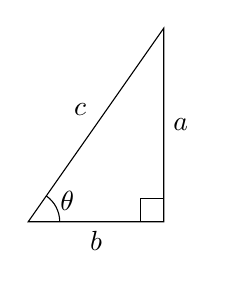
\begin{tikzpicture}[scale=3]
\coordinate (O) at (0,0);
\coordinate (P) at (55:1);
\coordinate (X) at (55:1 |- 0,0);
\draw[] (O) -- node[pos=0.5,above left]{$c$} (P) -- node[pos=0.5,right]{$a$} (X) -- node[pos=0.5,below]{$b$}(O) -- cycle;
\draw pic["$\theta$",draw,-,angle eccentricity=1.4, angle radius=0.4cm]{angle=X--O--P};
\draw pic["",draw,-,angle eccentricity=1.4, angle radius=0.3cm]{right angle=P--X--O};
\end{tikzpicture}
\raisebox{1cm}{\hspace{1cm}and\hspace{1cm}}
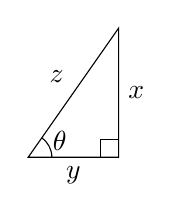
\begin{tikzpicture}[scale=2]
\coordinate (O) at (0,0);
\coordinate (P) at (55:1);
\coordinate (X) at (55:1 |- 0,0);
\draw[] (O) -- node[pos=0.5,above left]{$z$} (P) -- node[pos=0.5,right]{$x$} (X) -- node[pos=0.5,below]{$y$}(O) -- cycle;
\draw pic["$\theta$",draw,-,angle eccentricity=1.5, angle radius=0.3cm]{angle=X--O--P};
\draw pic["",draw,-,angle eccentricity=1.4, angle radius=0.225cm]{right angle=P--X--O};
\end{tikzpicture}
\end{center}

The sidelengths of one triangle are proportional to the side lengths of the other. This means that the ratio of two side lengths from one triangle and corresponding ratio on the other triangle are one in the same. In right triangles, you can express these ratios as functions of just one angle, since the other is given by the definition. The trigonometric functions do just this. For any angle theta, they output the side length ratio of the corresponding similar triangle.

\vspace{10pt}

{\bf{}Side Note}

\vspace{10pt}

Well, not exactly... but our later definition will be easier to grasp if we think of it this way for now. It is useful to tweak the definition a bit to make sense for non-acute angles. The unit circle definitions of the trig functions are more complete because, for example, instead of outputting the ratios of two side lengths of a triangle, the sine and cosine functions now output the $x$ and $y$ coordinates respectively of the point where the angle in standard position intersects the unit circle - allowing it to make sense for non-acute angles. Standard position means rotating counter-clockwise from the positive $x$-axis. I apologize if this is a bit wordy, I like to provide complimentary explanations in the form of writing and diagrams, and this concept requires a bit of setting up. The reason I'm mentioning this now is so that we can begin with the end in mind and understand each individual step we will take in the context of the larger whole.

\vspace{10pt}

So, pretending that we don't know where this is heading, we can define some primitive definitions of the trigonometric functions (corresponding to the figures above), and you will remember this from SOH CAH TOA:

\[\frac{a}{c}=\frac{x}{z}=\sin\theta\]

\[\frac{b}{c}=\frac{y}{z}=\cos\theta\]

\[\frac{a}{b}=\frac{x}{y}=\tan\theta\]

\[\cot\theta=\frac{b}{a}=\frac{y}{x}=\frac{1}{\tan\theta}\]

\[\sec\theta=\frac{c}{b}=\frac{z}{y}=\frac{1}{\cos\theta}\]

\[\csc\theta=\frac{c}{a}=\frac{z}{x}=\frac{1}{\sin\theta}\]

\newpage

After exploring the relationship between acute angles and their corresponding families of similar right triangles, we looked at the relationship between angles and their corresponding families of similar circlular sectors. Due to the families being similar, we can simplify things greatly by analyzing things in terms of a unit circle, then scaling our results up by the length of the radius. 

\vspace{10pt}

Anyways, for any given angle, any arc of a circle which subtends an angle of that magnitude is of equal length, regardless of which way the angle is oriented - see the figure below for a visual demonstration of this. Just to clarify, that little arrow which goes both ways is the formal mathematical notation for``if and only if".

\begin{center}
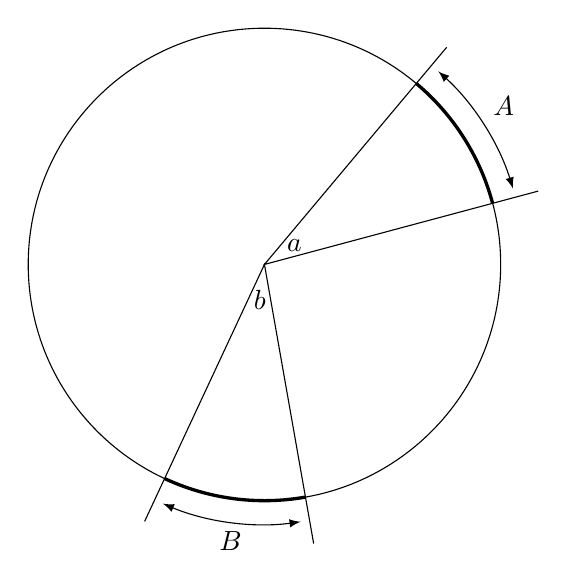
\begin{tikzpicture}[scale=3]
\coordinate (O) at (0,0);
\coordinate (C1) at (15:1.2);
\coordinate (C2) at (50:1.2);
\coordinate (C3) at (245:1.2);
\coordinate (C4) at (280:1.2);
\draw[] (O) circle [radius=1];
\draw[] (C1) -- (O) -- (C2);
\draw[] (C3) -- (O) -- (C4);
\draw pic["$a$",angle eccentricity=1.5, angle radius=0.3cm]{angle=C1--O--C2};
\draw pic["$b$",angle eccentricity=1.5, angle radius=0.3cm]{angle=C3--O--C4};
\draw[very thick] (15:1) arc [start angle=15, end angle=50, radius=1];
\draw[latex-latex] (17:1.1) arc [start angle=17, end angle=48, radius=1.1] node[pos=0.5,above right]{$A$};
\draw[very thick] (245:1) arc [start angle=245, end angle=280, radius=1];
\draw[latex-latex] (247:1.1) arc [start angle=247, end angle=278, radius=1.1] node[pos=0.5,below]{$B$};
\end{tikzpicture}
\end{center}

\[a=b\iff A=B\]

I should probably distinguish between a capital A or B, and a capital Alpha or Beta - Greek letters - for the next diagram... The english letters appear slanted or italisized, as in the above diagram, whereas capital Alpha and Beta are not slanted or italisized. Anyways, in the next diagram, we let the angle $r=1\textnormal{ rad}\approx57^\circ$, meaning the corresponding arc is the same length as the circle's radius.

\begin{center}
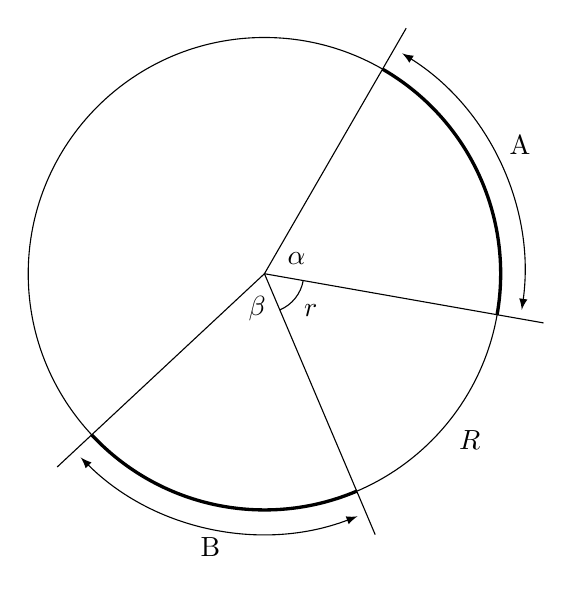
\begin{tikzpicture}[scale=3]
\coordinate (O) at (0,0);
\coordinate (C1) at (-10:1.2);
\coordinate (C2) at (60:1.2);
\coordinate (C3) at (223:1.2);
\coordinate (C4) at (293:1.2);
\draw[] (O) circle [radius=1];
\draw[] (C1) -- (O) -- (C2);
\draw[] (C3) -- (O) -- (C4);
\draw pic["$\alpha$",angle eccentricity=1.5, angle radius=0.3cm]{angle=C1--O--C2};
\draw pic["$\beta$",angle eccentricity=1.5, angle radius=0.3cm]{angle=C3--O--C4};
\draw pic["$r$",draw,-,angle eccentricity=1.5, angle radius=0.5cm]{angle=C4--O--C1};
\draw[very thick] (-10:1) arc [start angle=-10, end angle=60, radius=1];
\draw[latex-latex] (-8:1.1) arc [start angle=-8, end angle=58, radius=1.1] node[pos=0.5,above right]{$\mathrm{A}$};
\draw[very thick] (223:1) arc [start angle=223, end angle=293, radius=1];
\draw[latex-latex] (225:1.1) arc [start angle=225, end angle=291, radius=1.1] node[pos=0.5,below]{$\mathrm{B}$};
\path[] (293:1) arc [start angle=293, end angle=350, radius=1] node[pos=0.5,below right]{$R$};
\end{tikzpicture}
\end{center}

Similar to the previous diagram, the angles $\alpha$ and $\beta$ are the same, meaning their corresponding arclengths are also equal - due to belonging to similar circular sectors. The point of this diagram is to emphasize that the ratio of two separate angles is the same as the ratio of their corresponding arclengths. The reason we let $r=1\textnormal{ rad}$ is to demonstrate that any arclength is a scalar multiple of the radius, where the scalar multiple is its angle in radians. And to be clear, by $r$ we mean the angle measure in radians and not the radius which is still arbitrary.

\[\alpha=\beta\iff\mathrm{A}=\mathrm{B}\]

\[\frac{a}{r}=\frac{A}{R}=\frac{\textnormal{arc}}{\textnormal{radius}}=\textnormal{{\bf{}unitless} value}\]

If we let the radius equal to one - making it no longer arbitrary, then we a have a {\bf{}unit circle}.

\begin{center}
\begin{tikzpicture}[scale=3]
\draw[thick,-stealth] (0,-1.3) -- (0,1.3);
\draw[thick,-stealth] (-1.3,0) -- (1.3,0);
\coordinate (O) at (0,0);
\node[below left] at (O) {$O$};
\coordinate (P) at (34.377:1);
\coordinate (X) at (1,0);
\draw[] (O) circle [radius=1];
\draw[] (P) -- (O);
\fill[] (P) circle [radius=0.02];
\draw pic["$\alpha$",-latex,draw,angle eccentricity=1.5, angle radius=0.5cm]{angle=X--O--P};
\draw[latex-latex] (2:1.1) arc [start angle=2, end angle=32.377, radius=1.1] node[pos=0.5,right]{$\frac{\textnormal{arc}}{\textnormal{radius}}\approx0.6$};
\end{tikzpicture}
\end{center}

The arclength looks like it is about $0.6$, since the radius is $1$.

\[\frac{\textnormal{arc}}{\textnormal{radius}}\approx0.6\]

\begin{center}
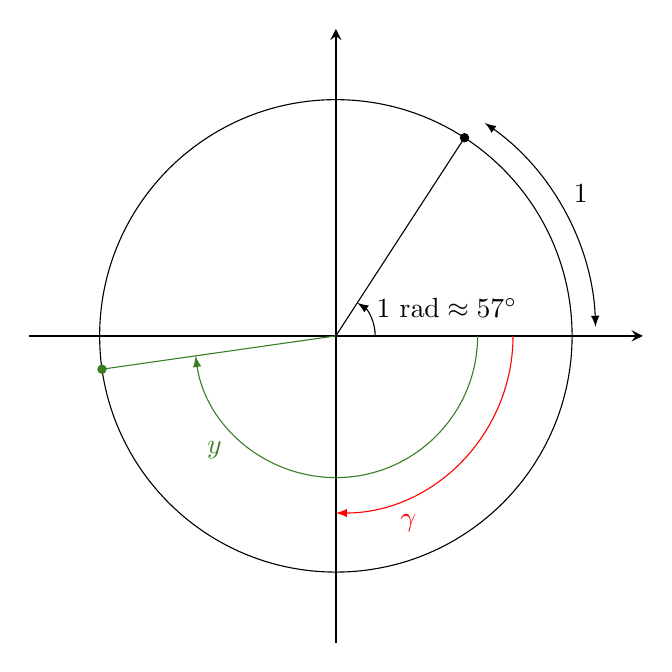
\begin{tikzpicture}[scale=3]
\draw[thick,-stealth] (0,-1.3) -- (0,1.3);
\draw[thick,-stealth] (-1.3,0) -- (1.3,0);
\coordinate (O) at (0,0);
\coordinate (P) at (57:1);
\coordinate (X) at (1,0);
\draw[] (O) circle [radius=1];
\draw[] (P) -- (O);
\fill[] (P) circle [radius=0.02];
\draw pic["\hspace{1.5cm}$1\textnormal{ rad}\approx57^\circ$",-latex,draw,angle eccentricity=1.5, angle radius=0.5cm]{angle=X--O--P};
\draw[latex-latex] (2:1.1) arc [start angle=2, end angle=55, radius=1.1] node[pos=0.5,above right]{$1$};
\draw[OliveGreen] (O) -- (-171.887:1);
\fill[OliveGreen] (-171.887:1) circle [radius=0.02];
\draw[-latex,OliveGreen] (0:0.6) arc [start angle=0, end angle=-171.887, radius=0.6] node[pos=0.8,below left]{$y$};
\draw[-latex,red] (0:0.75) arc [start angle=0, end angle=-90, radius=0.75] node[pos=0.8,below right]{$\gamma$};
\end{tikzpicture}
\end{center}

\[{\color{red}\gamma=\frac{-\pi}{2}}\qquad{\color{OliveGreen}y=-3}\]

As a final note, a central angle of $180^\circ$ is subtended by a special arc called a semicircle.

\vspace{10pt}

So there are two ``special" right triangles which we can geometrically analyze to obtain the exact trigonometric ratios of their angles. The right triangles in question are the $\angle30^\circ-60^\circ$ triangle, as well as the triangle corresponding to angles of $\angle45^\circ-45^\circ$.

\vspace{10pt}

Let us first examine the $\angle30^\circ-60^\circ$ triangle. We can reflect it to obtain an equilateral (or ``regular") triangle - something which we know the dimensions of, and which allows us to easily find the sidelengths of our special triangle using Pythagoras's Theorem:

\begin{center}
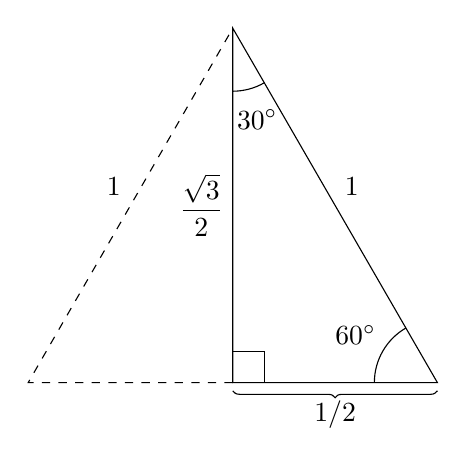
\begin{tikzpicture}[scale=3]
\coordinate (A) at (-30:1);
\coordinate (B) at (90:1);
\coordinate (C) at (210:1);
\coordinate (M) at (210:1 -| 0,0);
\draw[] (M) -- node[pos=0.5,left]{$\displaystyle\frac{\sqrt{3}}{2}$} (B) -- node[pos=0.5,above right]{$1$} (A) -- (M) -- cycle;
\draw[dashed] (M) -- (C) -- node[pos=0.5,above left]{$1$} (B);
\draw pic["",draw,angle eccentricity=1.5, angle radius=0.4cm]{right angle=A--M--B};
\draw pic["$30^\circ$",draw,angle eccentricity=1.5, angle radius=0.8cm]{angle=M--B--A};
\draw pic["$60^\circ$",draw,angle eccentricity=1.5, angle radius=0.8cm]{angle=B--A--M};
\draw [decorate, decoration = {brace,mirror,raise=3pt}] (M) --  (A) node[pos=0.5,below=3pt]{$1/2$};
\end{tikzpicture}
\end{center}

Having found the corresponding sidelengths to the angles, we can calculate their trigonometric ratios with precision:

\begin{align*}
\cos60^\circ&=\sin30^\circ=\frac{1}{2}\\
\sin60^\circ&=\cos30^\circ=\frac{\sqrt{3}}{2}\\
\tan60^\circ&=\cot30^\circ=\sqrt{3}
\end{align*}

The $45^\circ$ right triangle (which is called an "Isosceles Triangle") is easier to do this with because we can readily apply the Pythagorean Theorem:

\begin{center}
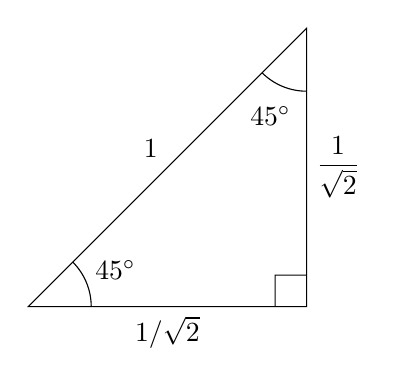
\begin{tikzpicture}[scale=5]
\coordinate (O) at (0,0);
\coordinate (P) at (45:1);
\coordinate (X) at (P |- O);
\draw[] (O) -- node[pos=0.5,above left]{$1$} (P) -- node[pos=0.5,right]{$\displaystyle\frac{1}{\sqrt{2}}$} (X) -- node[pos=0.5,below]{$1/\sqrt{2}$} (O) -- cycle;
\draw pic["",draw,angle eccentricity=1.5, angle radius=0.4cm]{right angle=P--X--O};
\draw pic["$45^\circ$",draw,angle eccentricity=1.5, angle radius=0.8cm]{angle=X--O--P};
\draw pic["$45^\circ$",draw,angle eccentricity=1.5, angle radius=0.8cm]{angle=O--P--X};
\end{tikzpicture}
\end{center}

\[\tan\frac{\pi}{4}=1\]

\[\sin\frac{\pi}{4}=\cos\frac{\pi}{4}=\frac{1}{\sqrt{2}}\]

Do note that when you are applying a trigonometric function to a number, that the number is implied to be in radians unless otherwise stated.

\vspace{10pt}

Now, as prophesized on the first page, we moved on to expanding the definitions of the trigonometric functions to make sense for arbitrary angles.

\begin{center}
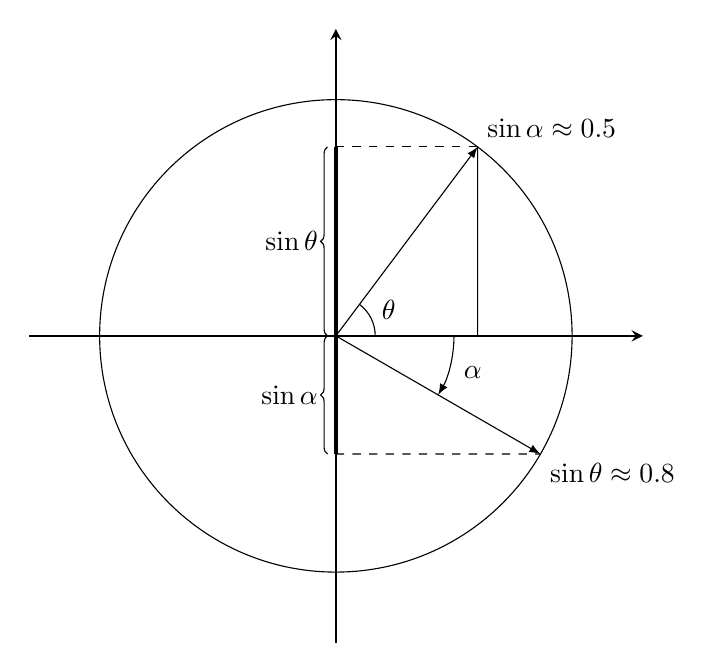
\begin{tikzpicture}[scale=3]
\draw[thick,-stealth] (0,-1.3) -- (0,1.3);
\draw[thick,-stealth] (-1.3,0) -- (1.3,0);
\coordinate (O) at (0,0);
\coordinate (P1) at (0.6,0.8);
\coordinate (X) at (P1 |- O);
\coordinate (P2) at (-30:1);
\coordinate (Y) at (P2 -| O);
\draw[] (O) circle [radius=1];
\draw[-latex] (O) -- (P1);
\draw[-latex] (O) -- (P2);
\draw pic["$\theta$",-,draw,angle eccentricity=1.5, angle radius=0.5cm]{angle=X--O--P1};
\draw pic["$\alpha$",latex-,draw,angle eccentricity=1.2, angle radius=1.5cm]{angle=P2--O--X};
\draw[] (P1) -- (X);
\draw[dashed] (Y) -- (P2) node [pos=1,below right]{$\sin\theta\approx0.8$};
\draw[dashed] (P1 -| O) -- (P1) node [pos=1,above right]{$\sin\alpha\approx0.5$};
\draw[very thick] (Y) -- (P1 -| O);
\draw [decorate, decoration = {brace,raise=3pt}] (O) -- (P1 -| O) node[pos=0.5,left=3pt]{$\sin\theta$};
\draw [decorate, decoration = {brace,raise=3pt}] (Y) -- (O) node[pos=0.5,left=3pt]{$\sin\alpha$};
\end{tikzpicture}
\end{center}

And what the diagram means to convery is that we are now defining the sine function to output the terminal $y$-coordinate of a unit-vector in the direction specified by the angle. In the same way, the cosine function outputs the terminal $x$-value of this unit-vector.

\vspace{10pt}

Below is a diagram which illustrates representing new angles as differences of other angles.

\begin{center}
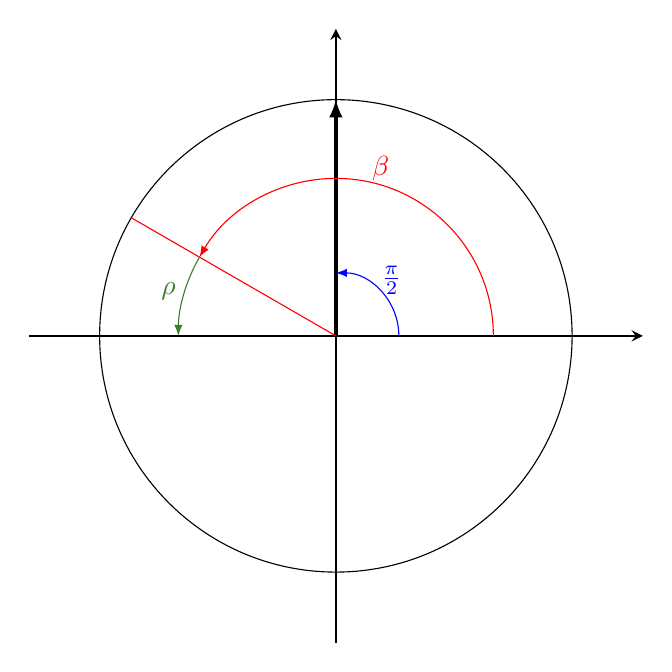
\begin{tikzpicture}[scale=3]
\draw[thick,-stealth] (0,-1.3) -- (0,1.3);
\draw[thick,-stealth] (-1.3,0) -- (1.3,0);
\coordinate (O) at (0,0);
\coordinate (P2) at (180:1);
\coordinate (P1) at (150:1);
\coordinate (Y) at (90:1);
\coordinate (X) at (0:1);
\draw[] (O) circle [radius=1];
\draw[-latex,very thick] (O) -- (Y);
\draw[-,red] (O) -- (P1);
\draw pic["$\beta$",-latex,draw,angle eccentricity=1.1, angle radius=2cm,red]{angle=X--O--P1};
\draw pic["$\rho$",-latex,draw,angle eccentricity=1.1, angle radius=2cm,OliveGreen]{angle=P1--O--P2};
\draw pic["$\frac{\pi}{2}$",latex-,draw,angle eccentricity=1.25, angle radius=0.8cm,blue,-latex]{angle=X--O--Y};
\end{tikzpicture}
\end{center}

\[{\color{OliveGreen}\rho=n\pi-\beta|n\textnormal{ is odd}}\]

And This graphic shows that a unit vector that is equal in magnitude but opposite in direction to another unit vector will have a sine which is equal in magnitude but opposite in sign.

\begin{center}
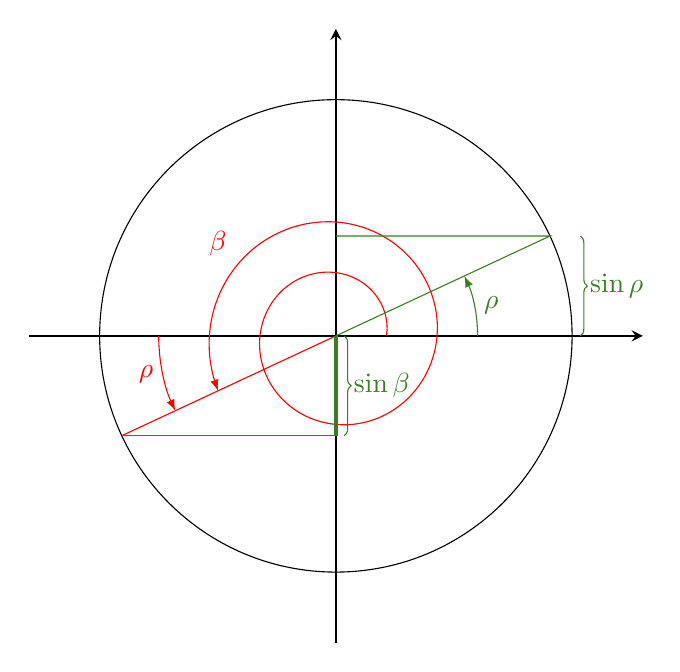
\begin{tikzpicture}[scale=3]
\draw[thick,-stealth] (0,-1.3) -- (0,1.3);
\draw[thick,-stealth] (-1.3,0) -- (1.3,0);
\coordinate (O) at (0,0);
\draw[] (O) circle [radius=1];
\draw[-latex,domain=360:925,variable=\t,smooth,samples=75,red] plot ({\t}: {0.0006*\t});
\node[above left] at (865:0.0006*865) {${\color{red}\beta}$};
\draw[red] (O) -- (925:1);
\draw[red,-latex] (-0.75,0) arc [start angle=180, end angle=205, radius=0.75] node[pos=0.5,left]{$\rho$};
\draw[OliveGreen] (O) -- (25:1) -- (0,0.42262);
\draw[OliveGreen] (925:1) -- (0,-0.42262);
\draw[OliveGreen,very thick] (O) -- (0,-0.42262);
\draw[OliveGreen,-latex] (0.6,0) arc[start angle=0, end angle=25, radius=0.6] node[pos=0.5,right]{$\rho$};
\draw [decorate,color=OliveGreen, decoration = {brace,mirror,raise=3pt}] (0,-0.42262) -- (O) node[pos=0.5,right=3pt,OliveGreen]{$\sin\beta$};
\draw [decorate,color=OliveGreen, decoration = {brace,mirror,raise=3pt}] (1,0) -- (1,0.42262) node[pos=0.5,right=3pt,OliveGreen]{$\sin\rho$};
\end{tikzpicture}
\end{center}

\[{\color{OliveGreen}\sin\beta=-\sin\rho}\]

\[{\color{OliveGreen}\rho=\beta-3\pi}\]

For some reason, we analyzed all of this in terms of sine, but the same reasoning applies to cosine, except it refers to the $x$-coordinate.

\begin{center}
\begin{tikzpicture}[scale=3]
\draw[thick,-stealth] (0,-1.3) -- (0,1.3);
\draw[thick,-stealth] (-1.3,0) -- (1.3,0);
\coordinate (O) at (0,0);
\coordinate (P) at (55:1);
\coordinate (X) at (P |- O);
\draw[] (O) circle [radius=1];
\draw[very thick] (O) -- (X);
\draw [decorate, decoration = {brace,mirror,raise=3pt}] (O) -- (X) node[pos=0.5,below=3pt]{$\cos\theta$};
\draw[-latex] (0.15,0) arc [start angle=0, end angle=55, radius=0.15] node[pos=0.5,right]{$\theta$};
\draw[] (O) -- (P);
\draw[dashed] (P) -- (X);
\end{tikzpicture}
\end{center}

And finally we wrapped up with a geometric demonstration of sine being an odd function, and cosine being an even function.

\begin{center}
\begin{tikzpicture}[scale=3]
\draw[thick,-stealth] (0,-1.3) -- (0,1.3);
\draw[thick,-stealth] (-1.3,0) -- (1.3,0);
\coordinate (O) at (0,0);
\coordinate (P1) at (130:1);
\coordinate (P2) at (-130:1);
\coordinate (X) at (P1 |- O);
\draw[-latex] (0.6,0) arc [start angle=0, end angle=130, radius=0.6] node[pos=0.35,above right]{$\alpha$};
\draw[-latex] (0.6,0) arc [start angle=0, end angle=-130, radius=0.6] node[pos=0.35,below right]{$-\alpha$};
\draw[] (O) -- (P1);
\draw[] (O) -- (P2);
\draw[very thick] (X) -- (O);
\draw [decorate, decoration = {brace,raise=3pt}] (X) -- (O) node[pos=0.5,above=3pt]{$\cos\theta\textnormal{ (both)}$};
\draw[dashed] (P1) -- (P2);
\draw[] (P2) -- (0,-0.76604) node[below,pos=0.5]{$\sin-\alpha$};
\draw[] (P1) -- (0,0.76604) node[above,pos=0.5]{$\sin\alpha$};
\end{tikzpicture}
\end{center}

We ended class with a warning against forgetting the scale of the diagram when graphing two functions.



\end{document}